\documentclass[10pt,a4paper]{article}

% ── Geometry: tight margins for note sheet ─────────────────────────────────
\usepackage[a4paper, top=0.9cm, bottom=0.9cm, left=1cm, right=1cm]{geometry}
\usepackage{graphicx}
\usepackage{float}
\usepackage{amsmath}
\usepackage{amssymb}
\usepackage{xcolor}
\usepackage{mdframed}
\usepackage{parskip}
\usepackage{enumitem}
\usepackage{titlesec}
\usepackage{multicol}
\usepackage{booktabs}
\usepackage{tikz}
\usetikzlibrary{arrows.meta, positioning, shapes.geometric}
\usepackage[T1]{fontenc}

\graphicspath{{../../reference/Network_extracted/figures/Lecture1/}}

% ── Colours ────────────────────────────────────────────────────────────────
\definecolor{keyblue}{RGB}{30, 80, 160}
\definecolor{keybluebg}{RGB}{220, 235, 255}
\definecolor{noteorange}{RGB}{200, 100, 0}
\definecolor{noteorangebg}{RGB}{255, 240, 215}
\definecolor{warnred}{RGB}{180, 30, 30}
\definecolor{warnredbg}{RGB}{255, 220, 220}
\definecolor{defgreen}{RGB}{20, 110, 50}
\definecolor{defgreenbg}{RGB}{215, 245, 225}
\definecolor{headernavy}{RGB}{25, 35, 90}

% ── Box environments ───────────────────────────────────────────────────────
\newmdenv[linecolor=keyblue,backgroundcolor=keybluebg,linewidth=1.5pt,
  leftline=true,rightline=false,topline=false,bottomline=false,
  innerleftmargin=7pt,innerrightmargin=6pt,
  innertopmargin=3pt,innerbottommargin=3pt,
  skipabove=3pt,skipbelow=3pt]{keybox}

\newmdenv[linecolor=noteorange,backgroundcolor=noteorangebg,linewidth=1.5pt,
  leftline=true,rightline=false,topline=false,bottomline=false,
  innerleftmargin=7pt,innerrightmargin=6pt,
  innertopmargin=3pt,innerbottommargin=3pt,
  skipabove=3pt,skipbelow=3pt]{notebox}

\newmdenv[linecolor=defgreen,backgroundcolor=defgreenbg,linewidth=1.5pt,
  leftline=true,rightline=false,topline=false,bottomline=false,
  innerleftmargin=7pt,innerrightmargin=6pt,
  innertopmargin=3pt,innerbottommargin=3pt,
  skipabove=3pt,skipbelow=3pt]{defbox}

\newmdenv[linecolor=warnred,backgroundcolor=warnredbg,linewidth=1.5pt,
  leftline=true,rightline=false,topline=false,bottomline=false,
  innerleftmargin=7pt,innerrightmargin=6pt,
  innertopmargin=3pt,innerbottommargin=3pt,
  skipabove=3pt,skipbelow=3pt]{warnbox}

% ── Section formatting ─────────────────────────────────────────────────────
\titleformat{\section}[block]{\normalsize\bfseries\color{headernavy}}{}{0pt}{}
  [\vspace{1pt}\rule{\linewidth}{0.6pt}\vspace{2pt}]
\titleformat{\subsection}[block]{\small\bfseries\color{keyblue}}{}{0pt}{}
\titlespacing*{\section}{0pt}{5pt}{2pt}
\titlespacing*{\subsection}{0pt}{3pt}{1pt}

% ── List spacing ───────────────────────────────────────────────────────────
\setlist{nosep, topsep=1pt, itemsep=1pt, leftmargin=1.3em}

\parskip=2pt
\parindent=0pt

% ===========================================================================
\begin{document}
% ===========================================================================

% ── Question header ─────────────────────────────────────────────────────────
\begin{center}
  {\large\bfseries\color{headernavy}%
    Q1 \textemdash{} Performance in Networked Systems \& Queueing Models}\\[1pt]
  {\small MM1 $\cdot$ Hans-Peter Schwefel}
\end{center}
\vspace{1pt}\hrule height 1pt\vspace{5pt}

% ── Meta intro ──────────────────────────────────────────────────────────────
Many different performance metrics exist in networks:
\begin{itemize}
  \item \textbf{Throughput} --- how much data gets through per second
  \item \textbf{Jitter} --- variation in packet delay
  \item \textbf{Utilisation} --- fraction of link capacity in use
  \item \textbf{Delay \& packet loss} --- how long packets wait and how often they are dropped
\end{itemize}
Of these, \textbf{delay} and \textbf{loss} are the most critical in packet-switched networks \\[4pt] 
Some of the Delay and Loss sources Are:
% ===========================================================================
\section*{1\quad Overview --- What \& Why}
% ===========================================================================


\vspace{3pt}

\begin{minipage}[t]{0.49\textwidth}
\textbf{Delay sources:}
\begin{itemize}
  \item Connection setup (TCP handshake)
  \item Queueing (waiting in buffer)
  \item Serialization (placing bits on wire)
  \item Medium access (CSMA, TDMA, \ldots)
  \item Retransmissions (lost frames)
\end{itemize}
\end{minipage}\hfill
\begin{minipage}[t]{0.49\textwidth}
\textbf{Loss sources:}
\begin{itemize}
  \item Buffer overflow (queue full $\to$ drop)
  \item Collisions (shared medium)
  \item Checksum/CRC mismatch
  \item (TCP) session drop
\end{itemize}
\end{minipage}

\vspace{3pt}
\begin{keybox}
  \begin{itemize}
    \item Unlike propagation or serialisation.
    \item Queueing delay is \emph{stochastic}:
    \begin{itemize}
    \item It varies with load and cannot be predicted by a simple formula. 
    \item This is why we model networks with \textbf{queueing theory}.
    \end{itemize} 
  \end{itemize}
\end{keybox}
\begin{notebox}
\textbf{Networks} are \emph{packet-switched}: packets share links and wait in
buffers $\Rightarrow$ \textbf{delay} and \textbf{loss}. We model this with
\emph{queueing theory} (Markov chains) to predict $\mathbb{E}[\text{delay}]$,
$P(\text{loss})$, throughput.
\end{notebox}
% ===========================================================================
\section*{2\quad Kendall Notation --- $X/Y/C\,[/B]$}
% ===========================================================================
To describe and classify queue types we use \textbf{Kendall notation} $X/Y/C\,[/B]$, where each symbol describes one aspect of the system:\\
\begin{minipage}[t]{0.52\textwidth}
\begin{defbox}
\begin{itemize}
  \item $X$ \textemdash{} Arrival process \quad (\textbf{M} = Markovian/Poisson)
  \item $Y$ \textemdash{} Service process \quad (\textbf{M} = exponential)
  \item $C$ \textemdash{} Number of servers
  \item $B$ \textemdash{} Buffer size (omit $\Rightarrow$ infinite)
\end{itemize}
\end{defbox}
\end{minipage}\hfill
\begin{minipage}[t]{0.45\textwidth}
  \begin{notebox}
    \textbf{Examples of these are} \\
\begin{tabular}{@{}ll@{}}
\toprule
Notation & Meaning \\\midrule
M/M/1 & 1 server, $\infty$ buffer \\
M/M/K/K & $K$ servers, $K$ buffer (blocking) \\
M/M/1/B & 1 server, finite buffer $B$ \\
\bottomrule
\end{tabular}
  \end{notebox}
\end{minipage}

% ===========================================================================
\section*{3\quad M/M/1 Queue}
% ===========================================================================
The simplest and most fundamental model is \textbf{M/M/1}:
\begin{itemize}
  \item \textbf{M} (arrival) --- memoryless Poisson process, rate $\lambda$; inter-arrival times are i.i.d.\ exponential
  \item \textbf{M} (service) --- memoryless exponential service times, rate $\mu$
  \item \textbf{1} --- single server; packets served one at a time (FCFS)
  \item infinite buffer.
\end{itemize}
\begin{keybox}
  
\textbf{Arrivals:} Poisson rate $\lambda$ \quad
\textbf{Service:} exp.\ rate $\mu$ \quad
\textbf{Utilization:} $\rho = \lambda/\mu$
\end{keybox}
\begin{warnbox}
Stable only if $\rho < 1$
\end{warnbox}

\vspace{4pt}

% ── Two representations side by side ────────────────────────────────────────
We can represent M/M/1 in two equivalent ways:
\begin{itemize} 
  \item \textbf{buffer+server diagram} showing the physical flow
  \item \textbf{birth-death chain} where each state $n$ is the number of packets currently in the system (waiting + being served).\\[3pt]
\end{itemize}
\begin{minipage}[t]{0.38\textwidth}
\small\textit{Buffer + server --- packets arrive, queue, get served:}
\vspace{6pt}

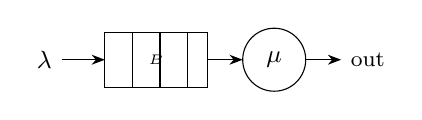
\begin{tikzpicture}[>=Stealth, font=\small]
  % Arrival arrow
  \draw[->] (0,0.35) -- (0.55,0.35);
  \node[left] at (0,0.35) {$\lambda$};
  % Buffer rectangle (split into cells)
  \draw (0.55,0) rectangle (1.85,0.7);
  \draw (0.9,0)  -- (0.9,0.7);
  \draw (1.25,0) -- (1.25,0.7);
  \draw (1.6,0)  -- (1.6,0.7);
  \node[font=\tiny] at (1.2,0.35) {$B$};
  % Arrow to server
  \draw[->] (1.85,0.35) -- (2.3,0.35);
  % Server circle
  \draw (2.7,0.35) circle (0.4);
  \node at (2.7,0.35) {$\mu$};
  % Output arrow
  \draw[->] (3.1,0.35) -- (3.55,0.35);
  \node[right, font=\footnotesize] at (3.55,0.35) {out};
\end{tikzpicture}
\end{minipage}\hfill
\begin{minipage}[t]{0.59\textwidth}
\small\textit{Birth-death chain --- state $n$ = \# packets in system (incl.\ in service):}
\vspace{4pt}

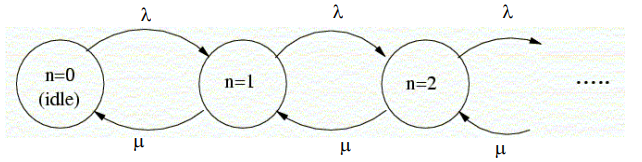
\includegraphics[width=\linewidth]{mm1queue.png}
\end{minipage}

\vspace{4pt}

% ===========================================================================
\section*{3b\quad M/M/1 --- Steady-State Results}
% ===========================================================================
\begin{minipage}[t]{0.52\textwidth}
\textbf{Steady-state distribution} (geometric):\\
The probability of finding exactly $i$ packets in the system:
\[
  \pi_i = \Pr(Q=i) = (1-\rho)\,\rho^i
\]
Probability server is idle: $\pi_0 = 1-\rho$
\end{minipage}\hfill
\begin{minipage}[t]{0.45\textwidth}
\textbf{Key metrics} ($Q$ = \# in system, $S$ = time in system):
\[
  \underbrace{\mathbb{E}[Q]}_{\text{avg.\ queue length}} = \frac{\rho}{1-\rho}, \qquad
  \underbrace{\mathbb{E}[S]}_{\text{avg.\ delay}} = \frac{1}{\mu-\lambda}
\]
Finite buffer $B$: $\;P_{\text{loss}} = \rho^B$
\end{minipage}

\vspace{3pt}
\begin{notebox}
\textbf{PASTA property:} Poisson arrivals see time averages ---
$P(\text{arrival finds } Q\!\ge\!B) = \Pr(Q\!\ge\!B) = \rho^B$
\end{notebox}

% ===========================================================================
\section{Extra Stuff (Pure Notes Don't say)}
\subsection*{Exercise: M/M/2 --- two servers, shared queue}

\begin{minipage}[t]{0.46\textwidth}
\small Arrival $\lambda$ feeds \emph{one} shared buffer; two servers each rate $\mu$.\\[3pt]
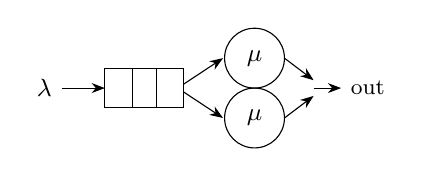
\begin{tikzpicture}[>=Stealth, font=\small]
  \draw[->] (0,0) -- (0.55,0);
  \node[left] at (0,0) {$\lambda$};
  \draw (0.55,-0.25) rectangle (1.55,0.25);
  \draw (0.9,-0.25)--(0.9,0.25);  \draw (1.2,-0.25)--(1.2,0.25);
  \draw[->] (1.55, 0.05) -- (2.05, 0.38);
  \draw[->] (1.55,-0.05) -- (2.05,-0.38);
  \draw (2.45, 0.38) circle (0.38); \node at (2.45,0.38) {$\mu$};
  \draw (2.45,-0.38) circle (0.38); \node at (2.45,-0.38) {$\mu$};
  \draw[->] (2.83, 0.38) -- (3.2, 0.1);
  \draw[->] (2.83,-0.38) -- (3.2,-0.1);
  \draw[->] (3.2,0) -- (3.55,0) node[right]{\footnotesize out};
\end{tikzpicture}

\vspace{3pt}
Birth-death --- death rate varies by state:\\
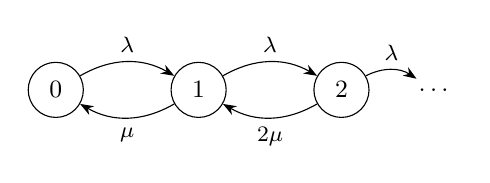
\begin{tikzpicture}[>=Stealth, font=\small, node distance=1.1cm]
  \node[draw,circle,minimum size=0.7cm] (s0) {0};
  \node[draw,circle,minimum size=0.7cm, right=of s0] (s1) {1};
  \node[draw,circle,minimum size=0.7cm, right=of s1] (s2) {2};
  \node[right=0.5cm of s2] (dots) {\ldots};
  \draw[->] (s0) to[bend left=30] node[above]{\footnotesize$\lambda$} (s1);
  \draw[->] (s1) to[bend left=30] node[below]{\footnotesize$\mu$}   (s0);
  \draw[->] (s1) to[bend left=30] node[above]{\footnotesize$\lambda$} (s2);
  \draw[->] (s2) to[bend left=30] node[below]{\footnotesize$2\mu$}  (s1);
  \draw[->] (s2) to[bend left=30] node[above]{\footnotesize$\lambda$} (dots);
\end{tikzpicture}
\end{minipage}\hfill
\begin{minipage}[t]{0.51\textwidth}
\begin{keybox}
\textbf{Note: increasing server speed always better}\\[3pt]
Compare three systems, same total capacity $2\mu$:
\begin{enumerate}[leftmargin=1.4em, itemsep=2pt]
  \item \textbf{M/M/1} rate $2\mu$ --- one fast server
  \item \textbf{M/M/2} rate $\mu$ each --- pooled queue
  \item \textbf{2$\times$M/M/1} rate $\mu$, split $\lambda/2$ each
\end{enumerate}
\[
  \mathbb{E}[S]_{\text{M/M/1},\,2\mu}
  \;<\;
  \mathbb{E}[S]_{\text{M/M/2},\,\mu}
  \;<\;
  \mathbb{E}[S]_{2\times\text{M/M/1},\,\mu}
\]
Pooling (shared queue) beats splitting.\\
A single faster server beats pooling.
\end{keybox}
\begin{notebox}
\small For M/M/2: $\rho = \lambda/(2\mu)$, death rate is $\mu$ in state 1, $2\mu$ in states $\ge2$.
\end{notebox}
\end{minipage}

\vspace{6pt}
% ===========================================================================
\section*{4\quad Birth-Death Process (General)}
% ===========================================================================

\begin{minipage}[t]{0.62\textwidth}
State = packets in system (queue \emph{+ in service}). Transitions only $\pm 1$.
M/M/1 is the simplest special case ($\lambda_k\!=\!\lambda$, $\mu_k\!=\!\mu$).

\textbf{General steady-state (product form):}
\[
  \pi_i = \pi_0 \prod_{k=0}^{i-1}\frac{\lambda_k}{\mu_{k+1}},
  \qquad
  \pi_0 = \left(1 + \sum_{i=1}^{\infty}\prod_{k=0}^{i-1}\frac{\lambda_k}{\mu_{k+1}}\right)^{-1}
\]
\end{minipage}\hfill
\begin{minipage}[t]{0.35\textwidth}
\begin{keybox}
\textbf{Flow balance} (global):
\[\mu_i\,\pi_i = \lambda_{i-1}\,\pi_{i-1}\]
Rate out of state $i$ = rate into state $i$.
\end{keybox}
\end{minipage}

% ===========================================================================
\section*{5\quad M/M/K/K Queue --- Erlang-B (Circuit Switching)}
% ===========================================================================

$K$ channels (servers). Call \textbf{blocked} (lost) if all $K$ busy --- no waiting room.
Departure rate from state $i$: $i/T$.

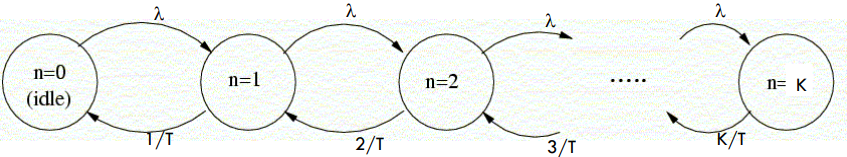
\includegraphics[width=0.88\linewidth]{MMKK.png}

\begin{notebox}
Death rate from state $i$ is $i/T$ because each of the $i$ active calls ends independently at rate $1/T$. Blocking probability $P_B = \pi_K$ --- the \textbf{Erlang-B} formula.
\end{notebox}

% ===========================================================================
\section*{6\quad M/M/1/K --- Finite Buffer}
% ===========================================================================

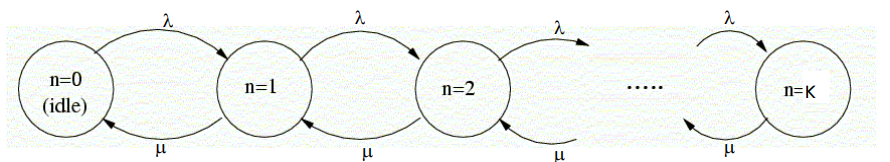
\includegraphics[width=0.75\linewidth]{MM1K.png}

\vspace{2pt}
\begin{minipage}[t]{0.55\textwidth}
\[
  \pi_i = \frac{1-\rho}{1-\rho^{K+1}}\,\rho^i \;(i=0,\ldots,K),
  \qquad
  P_{\text{loss}} = \pi_K
\]
\end{minipage}\hfill
\begin{minipage}[t]{0.42\textwidth}
\[
  \bar{D} = \frac{1}{\lambda(1-P_{\text{loss}})}\cdot
  \frac{\rho}{1-\rho^{K+1}}\!\left[\frac{1-\rho^K}{1-\rho} - K\rho^K\right]
\]
\end{minipage}

\end{document}
